\label{sec:reco-jets}
Hadrons produced in collisions usually decay before they reach the detectors. Because of the initial momentum of the hadron, the decay products travel in the same direction and form a cone which is known as jet. Reconstruction of jets uses single particles as inputs. The most widely used type of jets is calorimeter jets which faithfully represent the original hadron and uses calorimeter clusters as surrogates of single particles.

Energy deposits in calorimeter cells are first grouped into 3-D clusters called topological clusters (topocluster)\cite{PERF-2014-07}. We first form proto-clusters at the EM energy scale. The cells which pass a signal to noise significance $\sigma=\frac{E^{em}}{\sigma}$ thresholds are considered to belong to a cluster. The clustering algorithm starts with the seeds of $\sigma>4$ and then collects topologically connected (in the same layer adjacent or in two adjacent layers but have $\eta- \phi$ overlap) cells which are $\sigma>2$ and their direct neighbors with $\sigma>0$. Large clusters may lead to bad jet resolutions and are hence splitted if more than local maxima exists with $E^{EM}>500 \mev$ with certain spatial and layer constraints.

Many jet clustering algorithms exist. The most widely used algorithm within ATLAS is a sequential algorithm called anti-$k_t$\cite{Cacciari:2008gp}. The jet shape formed by this algorithm is not affected by soft radiations and making all the jet objects as conical as shown in Fig.\ref{fig:reco-antikt}. The algorithm treats clusters as input pseudo jets and calculates two metrics between two pseudo jets $i,j$: $d_{ij}=min(k^{-2}_{ti},k^{-2}_{tj})(\frac{\Delta^2_{ij}}{R^2})$ and $d_{iB}=k^{-2}_{ti}$, where $\Delta^2_{ij}=(y_i^2-y_j^2)+(\phi_i^2-\phi_j^2)$ and $k_t$ is the transverse momentum. If a pseudo jet is closer to the beam than to any other particle by these metrics then it is left alone. Otherwise, we combine it with its nearest neighbor as as a single pseudo-jet adding together their momenta. The clustering algorithm continues until no pseuodo jets can be combined.

\begin{figure}[htpb!]
\begin{center}
  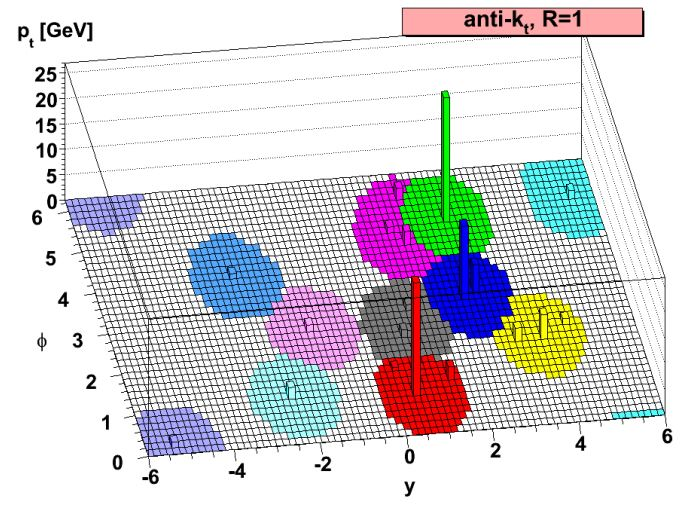
\includegraphics[width=0.55\linewidth]{figures/Reco/Antikt}
\caption{Illustration of jets clustered by anti-$k_t$ algorithm. The jet shapes are regular and conical}
\label{fig:reco-antikt}
\end{center}
\end{figure}

Jets require more dedicated correction of its four momenta than any other objects. ATLAS apply a series corrections\cite{PERF-2016-04} to jets in steps. First $|\eta|$ resolution is improved by using event primary vertex as jet origin. Pile-up contamination is corrected in the next step. Then MC based four momenta correction as well as jet initial content corrections are applied. Jets in data also receive \textit{in situ} calibration which corrects the difference between MC and data.

While the calorimeter jets gives a full representation of the initial hadron, another representation called track jets is very useful especially for identifying heavy flavor objects. The track jets are formed using tracks with a very loose selection on the impact parameters as ingredients to include tracks coming from secondary vertices. Only with a change of the input objects, all algorithms applicable to clustering calorimeter jets can be used for track jets clustering. While the track jets energy measurement is not interesting as it is on average $\frac{2}{3}$ of the initial hadron, it provides good angular resolution. 
